% !TEX spellcheck = en_US
\documentclass[letter,12pt]{article}
\usepackage{fancyhdr}
\usepackage{setspace}
\usepackage{fullpage}
\usepackage{amsmath}
\usepackage{amsfonts}
\usepackage{amssymb}
\usepackage{xfrac}
\usepackage{tikz}

\pagestyle{myheadings}
\markright{\hfill \textup{Maluff} }
\headsep 0.3in
\topmargin -0.3in
\textheight 9in

\newcommand{\N}{\mathbb{N}}
\newcommand{\Z}{\mathbb{Z}}
\newcommand{\Q}{\mathbb{Q}}
\newcommand{\R}{\mathbb{R}}
\newcommand{\C}{\mathbb{C}}
\newcommand{\F}{\mathbb{F}}

\doublespacing
\begin{document}

\begin{singlespace}
\noindent MATH \#\#\#-\#: Class name

\noindent Prof. Name Lastname

\noindent Mauricio Maluff Masi

\noindent 03/04/2012
\end{singlespace}
{\centering
\large{\textbf{Assignment 1}}

}
\vspace{12pt}
\noindent\textbf{1.1.2} 11, 15. \textbf{1.1.3} 8.

\noindent\textbf{1.1.2} 11. Prove that an edge $e$ is a bridge of $G$ if an only if $e$ lies on no cycle of $G$.\\

{\centering
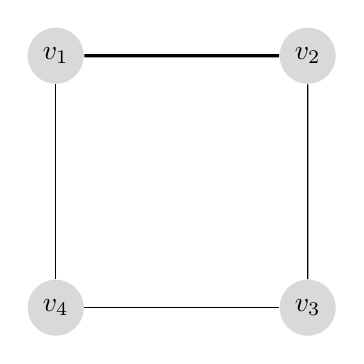
\begin{tikzpicture}
  [scale=.8,auto=left,every node/.style={circle,fill=gray!30}]
  \node (n4) at (1,1)  {$v_4$};
  \node (n3) at (5,1)  {$v_3$};
  \node (n2) at (5,5)  {$v_2$};
  \node (n1) at (1,5)  {$v_1$};

  \foreach \from/\to in {n2/n3,n3/n4,n4/n1}
  \draw (\from) -- (\to);
  \draw[very thick] (n1) -- (n2);

\end{tikzpicture}

}

































\end{document}
